% Section 6: Full-scan inversion and scoring. Facts: log blind pipeline (v3 inversion), items 56-59, 89-92, 104-108; figure F7.
\section{Full-scan inversion and scoring}\label{sec:fullscan}
\begin{notes}
\item Inversion: thickness only, $h = h_{\min} + (\SI{10}{mm} - h_{\min})\,e^{m}$ with $h_{\min}=1$\,mm, mass follows $\rho h$; $m$ on a 3\,mm grid ($100\times66$) over the scan area, bilinear onto the 1\,mm grid; loss = mean over shots of the normalised residual energy + TV ($10^{-4}$); Adam, learning rate 0.03, 100 updates from the blind background (converged by 75--100). The cube is not in the model (unknown target).
\item Full-scan maps with 4, 2 and 1 shots (F7): all five features found; 29 / 34 / 3 false indications. The model renders M1 and D3 as stiff plugs with a thin ring (no void, no glued mass in a plate model).
\item Philosophy: an unmodelled feature must at least be located and contained.
\end{notes}
\begin{figure}[ht]\centering
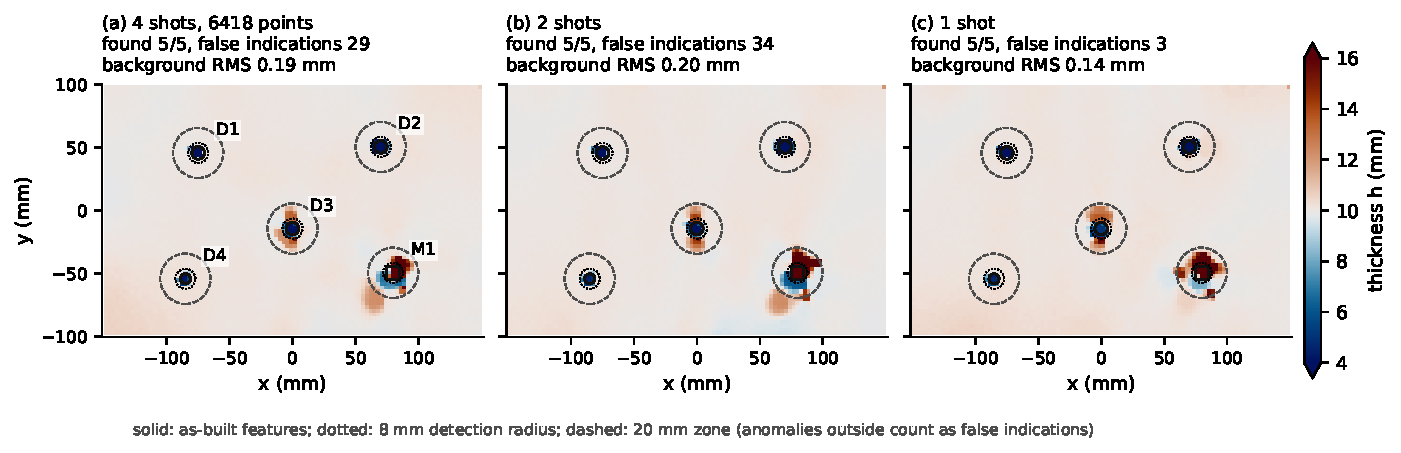
\includegraphics[width=\linewidth]{F7_fullscans.pdf}
\caption{\textbf{Blind full-scan inversions} with 4, 2 and 1 shots, and the scoring geometry (8\,mm detection radius, 20\,mm false-alarm zone). All five features are found in every case; the cube M1 and the through-hole D3 appear as stiff plugs with a thin ring.}\label{fig:fullscans}
\end{figure}


\subsection{Scoring}\label{sec:scoring}
\begin{notes}
\item Fixed-amplitude rule (pre-registered, internal name v3): anomaly $a=|h-\SI{10}{mm}|$; found if $a>3$\,mm within 8\,mm of the feature (all five, including M1); localisation error = distance to the peak of $a$ within 25\,mm; false indications = cells with $a>1$\,mm farther than 20\,mm (about half an A0 wavelength) from every feature, inside $|x|<140$, $|y|<90$\,mm; background RMS on the same cells; spill radius of M1 and D3. Ranking: found, then false indications, then background RMS. Term ``false indication'' (ASTM E1316).
\item Sensitivity (log items 90, 92): threshold 1.5--3\,mm and detection radius 4--20\,mm do not change the conclusions; say so in one sentence.
\item Fixed false-indication rate rule (exploratory): threshold of each map = 99th (95th) percentile of $a$ over the background cells, so every map has 1\,\% (5\,\%) false indications and methods differ only in detection (CFAR-type rule, common in NDT/radar). Motivation: sparse inversions underestimate amplitudes; D4 is often located correctly but below 3\,mm (log item 89).
\item \textbf{Defect-free-background argument}: in practice the background distribution would be obtained from a scan of a defect-free plate (or a defect-free region), inverted with the same layout and settings; here the cells more than 20\,mm from every feature play that role. State the limitation: a pristine-scan inversion may have a different background level than the damaged plate (scattered-field artefacts); a blind variant (whole-map percentile) weakens the 30-point results (log item 107) -- report in the appendix.
\item Why both rules are shown: the amplitude rule is pre-registered; the rate rule separates detection from amplitude calibration.
\end{notes}
